%%%%%%%%%%%%%%%%%%%%%%%%%%%%%%%%%%%%%%%%%
% Design based on a template by Roberto and following the format of
% the xmipp tutorials. In turn, they seem to be based on a template
% from http://www.latextemplates.com
%%%%%%%%%%%%%%%%%%%%%%%%%%%%%%%%%%%%%%%%%

%----------------------------------------------------------------------------------------
%	PACKAGES AND OTHER DOCUMENT CONFIGURATIONS
%----------------------------------------------------------------------------------------

\documentclass[12pt]{article} % Default font size is 12pt, it can be changed here
\usepackage[english]{babel}
\usepackage[utf8]{inputenc}
\usepackage{listings} % To include source code
\usepackage{caption}
\usepackage{subcaption}
\usepackage[htt]{hyphenat}
\usepackage{geometry} % Required to change the page size to A4
%\geometry{a4paper} % Set the page size to be A4 as opposed to the default US Letter
\usepackage{framed}
\usepackage{url}
\usepackage{graphicx} % Required for including pictures
\usepackage{natbib}
\usepackage{float} % Allows putting an [H] in \begin{figure} to specify the exact location of the figure
%\usepackage{hyperref}
\usepackage{menukeys}
\usepackage{array}
\usepackage{fancyhdr}
\usepackage{marvosym}%smileys\Smiley{} \Frowny{}
\usepackage{etoolbox}
\usepackage{listings}
\usepackage{makecell}
\usepackage{marginnote}
\usepackage{soul}
\usepackage[toc,page]{appendix}
\usepackage{caption}
\usepackage{menukeys}
\usepackage{fancybox,framed}
\usepackage{xspace}
\usepackage{rotating}
\usepackage{gensymb}
\usepackage{vhistory}

%commands
\newcommand{\ffigure}[1]{{Fig. {\ref{#1}}}\xspace}
\newcommand{\ttable}[1]{{Table {\ref{#1}}}\xspace}
\newcommand{\scommand}[1]{{{\keys{#1}}}\xspace}
%definitions
\def\ccmask{CC\textsubscript{MASK}\xspace}
\def\ccp4{\textit{CCP4}\xspace}
\def\chimera{\textit{Chimera}\xspace}
\def\coot{\textit{Coot}\xspace}
\def\emringer{\textit{EMRinger}\xspace}
\def\modeller{\textit{Modeller}\xspace}
\def\molprobity{\textit{MolProbity}\xspace}
\def\validationCryoEM{\textit{Validation CryoEM}\xspace}
\def\phenix{\textit{PHENIX}\xspace}
\def\powerfit{\textit{PowerFit}\xspace}
\def\refmac{\textit{Refmac}\xspace}
\def\scipion{\textit{Scipion}\xspace}
\def\scipiont{{scipion3}\xspace}

\sethlcolor{yellow}

%\renewcommand{\hl}[1]{#1}
%pdflatex -jobname=students '\def\student{}\input{main}'
%pdflatex -jobname=teachers '\def\teachers{}\input{main}'
%  \ifdef{\teachers}
%  {Content for teachers}
%  {Content for students} 
\newcommand{\ttt}[1]{\texttt{#1}}
\newcommand{\iii}[1]{\textit{#1}}
\newcommand{\ra}{$\rightarrow$}
\pagestyle{fancy}
\fancyhf{}
\fancyhead[RO]{{Developer's course: using images}}
\fancyhead[LO]{Scipion}
%\fancyhead[RO]{{\leftmark}}
\fancyfoot[RO]{\thepage}

\linespread{1.2} % Line spacing

%\setlength\parindent{0pt} % Uncomment to remove all indentation from paragraphs

\newenvironment{command}{\tt\begin{quote}}{\end{quote}}
\newcommand{\comm}[1]{\texttt{#1}}

\newcommand{\imgfig}[3]{\begin{figure}[H]\centering \
\includegraphics[scale=#2]{images/#1} \caption{#3} \end{figure}}

\newcommand{\proto}[1]{\textit{\textbf{#1}}}
\newcommand{\popt}[1]{\textit{#1}}
\newcommand{\pval}[1]{\texttt{#1}}
\def\repository{\ttt{scipion-em-template}\xspace}
\def\branch{\ttt{day3rmarabini}\xspace}
\def\protocolname{\ttt{protocol\_statistics}\xspace}

\newcommand\tstrut{\rule{0pt}{2.4ex}}
\newcommand\bstrut{\rule[-1.0ex]{0pt}{0pt}}

\def \humanAdenoMap {7034}%5172

\begin{document}

%----------------------------------------------------------------------------------------
%	TITLE PAGE
%----------------------------------------------------------------------------------------

\begin{titlepage}

% New command for horizontal lines. Change thickness here.
\newcommand{\HRule}{\rule{\linewidth}{0.5mm}}

\center % Center everything on the page


\includegraphics{images/scipion_logo}

{\large \scipion Developers Course}\\[1.0cm]

\textsc{\LARGE National Center for Biotechnology}\\[0.5cm]
\textsc{\Large Biocomputing Unit}\\[0.15cm]

\HRule\\[0.3cm]
{ \huge \bfseries \scipion Developers Course:  \\ Sets of Particles}\\ % Title of your document
\HRule \\[0.35cm]
{\large \today}\\ % Date, change the \today to a set date if you want to be precise
\begin{center}
\includegraphics[width=0.50\textwidth]{{images/virus.png}}\\
3D phantom of an icosahedral virus.
\end{center}

%\vfill % Fill the rest of the page with whitespace
%\begin{minipage}{0.4\textwidth}
\begin{flushright}
 \large
%\emph{Author:}\\
  \textsc{Roberto Marabini} % Your name
\end{flushright}
%\end{minipage}

\end{titlepage}

\begin{versionhistory}
%  \vhEntry{1.0}{10.15.2020}{MM|RM}{created for first developers workshop}
  \vhEntry{1.0}{10.15.2020}{RM}{created for first developers workshop}
\end{versionhistory}\newpage

%----------------------------------------------------------------------------------------
%	OBJETIVOS
%----------------------------------------------------------------------------------------
%----------------------------------------------------------------------------------------
%	TABLE OF CONTENTS
%----------------------------------------------------------------------------------------

\tableofcontents % Include a table of contents

\newpage % Begins on a new page instead of on the same page as the table of contents


\section{Setup and requeriments}
\subsection{Intended audience}
This guide has been tailored to developers who wish to program using the \scipion 
framework and have basic knowledge of software architecture and Python programming language. 

\subsection{We'd like to hear from you}

We have tested and verified the different steps described in this guide
to the best of our knowledge, but since our programs are in continuous
development you may find inaccuracies and errors in this text. Please
let us know about any errors, as well as your suggestions for
future editions, by writing to
scipion@cnb.csic.es.


\subsection{Requirements}

This tutorial requires \scipion with the \textit{xmipp\_bundle} installed. Basic knowledge of python is assumed.


\section{Practical Session}
\subsection{Objectives and Introduction}
%This guide will introduce the different tools and classes needed to handle sets of particles in \scipion.

%The basic idea underlying modular design is to organize a complex system (such as \scipion) as a set of components that can be developed independently and then plugged together. As in science in general, breaking a problem down to smaller, bite-sized pieces makes it easier to solve. It also allows different people to solve different parts of the problem and still have it all work correctly in the end. Each component is then self-contained and, as long as the interface between different components remains constant, can be extended or even gutted and rewritten as needed without causing a chaotic mess. 

In this practical session you will get familiar with the abstraction layer that provides to \scipion developers with an unified interface for accessing and manipulating an image (or set of images). This layer is responsible for translating the commands provided by the programmer into the specific format dependent commands needed by each particular image format.

The session has been divided in two parts. In the first one you will learn how to manipulate images and in the second we will address the problem of file format conversion.

Before going ahead I would like to warn you that, in \scipion,  the word ``image''  is used in different contexts with three different meanings:

\begin{itemize}
 \item Binary file storing the value of a collection of pixels. 
 \item Object of the class \ttt{Image} containing metada related to a ``binary file''.
 \item Object returned by the class \ttt{ImageHandler} that allows \scipion developers to access to a ``binary file'' using an API which does not depend on the file format.
\end{itemize}

\subsection{The data}

   In this practical session we are going to use a $120\times120\times120$ phantom (an artificial object) and 10 noisy projections along the same projection direction. Images are in the directory \ttt{data} (from the plugin-em-template root).
   
   \begin{itemize}
    \item {\bf virus.map:} 3D phantom, see surface rendering at figure~\ref{fig:rendering}
    \item {\bf proj.stk:} 10 noisy projections at the same angle figure~\ref{fig:proj}
   \end{itemize}

\begin{figure}[H]
\centering 
\includegraphics[scale=.2]{images/virus.png} 
\caption{surface rendering of a 3D phantom} 
\label{fig:rendering}
\end{figure}
\begin{figure}[H]
\centering 
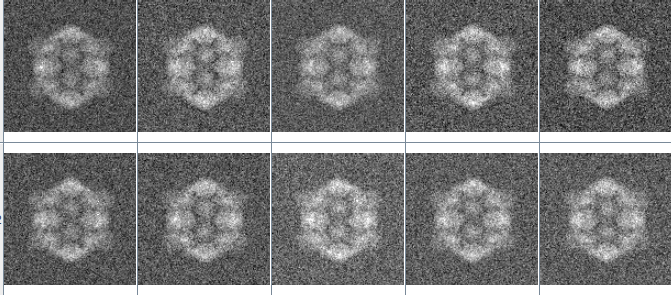
\includegraphics[scale=1]{images/proj.png} 
\caption{Galley of 10 noisy projections along the same projection direction.} 
\label{fig:proj}
\end{figure}

\subsection{Playing with the images}

Before creating a real protocol let us play a bit with the image API. In an object of type \ttt{Image} you can only store metadata related with the image as can be the name of the binary file in which the pixel values are stored, the sampling rate, information related with alignment, etc. Let us add the sampling rate and the name of the binary file to the \ttt{Image} object.

\begin{lstlisting}[language=Python, caption={The following script creates an object of the class \ttt{Image}.}]
$ scipion3 python # start python inside scipion3
>>> from pwem.objects.data import Image
>>> i = Image()
>>> i.setFileName('myImage.map')
>>> i.setSamplingRate(3.) # sampling rate in A
>>> for a in i.getAttributes(): # print all the pairs (key, value) 
                                # stored in the Image i
...    print(a[0], a[1].get())
_index 0
_filename myImage.map
_samplingRate 3.0

\end{lstlisting}

On the other hand the class \ttt{ImageHandler} actually accesses binary files and can modify them. In the following
example we are going to access a file and modify its content.

\begin{lstlisting}[language=Python, caption={The following script creates a $3\times3$ binary image using \ttt{ImageHandler}}]

>>> import numpy as np
>>> from pwem.emlib.image import ImageHandler # module to handle images
>>> fileName = 'three_by_three.mrc' # an small 3x3 image located
>>> ih = ImageHandler()
>>> image = ih.createImage() #  Uninitialized image of class xmipp.Image
>>> matrix = np.array([[1, 2, 3], [4, 5, 6], [7,8,9]], np.float32)
>>> image.setData(matrix)
>>> image.write("tmp.mrc")
>>> help(image) # list of image methods

# type in the terminal od -f tmp.mrc
# to see the content of file tmp.mrc
# you should see the header followed
# by the matrix
\end{lstlisting}


\subsection{Create a protocol that compute the mean and variance of a set of images}

Let us start with the real work. We are going to create a protocol that reads a set of particles (\ttt{proj.stk}, figure~\ref{fig:proj}) and computes the average and standard deviation images. The output should look like figure~\ref{fig:average} and figure~\ref{fig:variance}


\begin{figure}[H]
\centering 
     \begin{subfigure}[b]{0.3\textwidth}
         \centering
         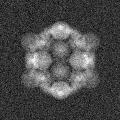
\includegraphics[width=\textwidth]{images/average.jpg}
         \caption{average image}
         \label{fig:average} 
     \end{subfigure}
     %\hfill
     \begin{subfigure}[b]{0.3\textwidth}
         \centering
         
\includegraphics[width=\textwidth]{images/variance.jpg}
         \caption{variance image}
         \label{fig:variance}
     \end{subfigure}
     \caption{The two images created by the protocol \ttt{Statistics}}
\end{figure}

We suggest you to follow a Test-Driven Development (TDD) approach, which is an approximation to codding where you write a test before you write just enough production code to fulfill that test. Therefore, TDD is one way to think through your requirements or design before your write your functional code.

Very likely you have downloaded the \repository repository (otherwise do it using the command \ttt{git clone https://github.com/scipion-em/scipion-em-template.git; cd scipion-em-template}). Update it (\ttt{git pull}) and switch to the branch called \branch (\ttt{git checkout tags/3\_1.statistics\_protocol\_template}, you may need to fetch it first with \ttt{git fetch --all --tags}). In this branch you will find a new protocol called \protocolname with the corresponding test. This protocol reads a \ttt{setOfParticles}, does nothing with them and creates as output two \ttt{Images}. These \ttt{Images} are empty in the sense that they do not point to any binary file. Execute the test \ttt{scipion3 tests myplugin.tests.test\_protocol\_statistics}, open \scipion (\ttt{scipion3 last}) and double check that a new project called \ttt{TestStatistics} has been created and that it contains two protocols called \ttt{import particles} and \ttt{compute statistics} respectively.

Now your work starts. You need to compute the average and variance image. Average images are created by adding together many pictures. If the images being averaged contain some commonalities, a pattern emerges revealing the regularities existing in the intensity patterns across all the images. On the other hand the variance images highlights those areas in which the differences are greater.

The steps you will need to fulfill are:
\begin{itemize}
 \item execute the test, it will complain that the images \ttt{average.mrc} and \ttt{variance.mrc} do not exists
 \item modify the code as described in the following steps so that this two files are created
 \item get the \ttt{setOfImages} from the input parameters (self.inputParticles.get())
 \item get image dimensions and number of images (\ttt{self.inputParticles.getDim()} and \ttt{self.inputParticles.getSize()} are your friend here)
 \item create two numpy arrays for the average and variance images. (\ttt{numpy.zeros([xdim, ydim]), numpy.float32})
 \item iterate through all particles (\ttt{for particle in self.inputParticles:})
 \item using particle \ttt{ ImageHandler().read(particle.getLocation())} read image and extract matrix (\ttt{getData}).
 \item the value of the average image at pixel $(i,j)$ is $\mu(i,j)=\frac {1}{N}\sum _{n=1}^{N}x_n(i,j)$. Where $N$ is the number of images and $x_n(i,j)$ the value of the pixel $(i,j)$ for the image $x_n$.
 \item the value of the variance image at pixel $(i,j)$ is\\ $\sigma^2_n(i,j)={ {{\frac {1}{N}}\sum _{n=1}^{N}\left(x_n(i,j)-{\mu(i,j)}\right)^{2}}}$. (see appendix~\ref{app:variance} for an algorithm to compute the variance in a computationally efficient way).
 \item assign the np.arrays to two \ttt{xmipp.Image} (\ttt{setData})
 \item and save them in the directory protocol extra directory (\ttt{self.\_getExtraPath(filename)}) with file names \ttt{average.mrc} and \ttt{variance.mrc} respectively.
 \item finally, assign the created filenames to the Two \ttt{Images} in the \ttt{createOutputStep} function
 \item Note that the default ``Analyze'' which shows all images produced by the protocols is just what we need in this case.
\end{itemize}

Remember: (1)  you may execute the protocol at any time running the test and in case you introduce
any print statement to debug your code the output will be redirected to the \scipion output log, (2) The solution
to this exercise can be browsed in github.com project scipion-em:scipion-em-template selecting the tag \ttt{3\_2.statistics\_protocol\_solution},


\subsection{Protocols that require image format conversion}
Some image processing software can only read a limited set of file formats.
Since we are using \ttt{ImageHandler} for reading, our protocol is quite tolerant from the image format point of view
but this is not always true and, when using third party software, many times we need to convert the data before it can be 
used as input. Let's imagine that we want to create a thumbnail of our image. 

A possible solution is to use the python PIL module:

\begin{lstlisting}[language=Python, caption={The following script creates  64x64 thumbnails using PIL.}, label={lst:PIL}]
>>> from PIL import Image # this is PIL Image class 
                          # not scipion Image class
>>> im = Image.open("tmp.jpg")
>>> size = 64, 64
>>> im.thumbnail(size)
>>> im.save("out.jpg")
\end{lstlisting}
%>>> image_pil_thr.save("out.spi", format='spider')
but unfortunately \ttt{PIL} will not read electron microscopy images. Therefore, we need to convert the image
before calling \ttt{PIL}. 

Reusing the protocol we just created (\ttt{statistics}) modify it so a thumbnail is created for each input particle and saved in an output stack. I have created a test file for you. You may execute it by typing: \ttt{scipion3 tests myplugin.tests.test\_protocol\_thumbnail}. Since the protocol has not been implemented, the test will fail. In order to pass the test you will need to:

\begin{itemize}
 \item make a copy of the file \ttt{protocol\_statistics.py} and call it \ttt{protocol\_thumbnail.py}
 \item change the \ttt{\_label} from \ttt{Statistics} to \ttt{Thumbnail}
 \item change the name of the class from \ttt{ProtStatistics} to \ttt{ProtThumbnail}
 \item import the new class in the \ttt{\_\_init\_\_.py}
 \item add an extra parameter to the protocol: the size of the output thumbnail (parameter type = \ttt{IntParam}, parameter name = \ttt{size})
 \item rename the function \ttt{computeStatistics} to \ttt{computeThumbnail}. Clean it, you only need to keep the lines 
\begin{lstlisting}[language=Python]
        setOfParticles = self.inputParticles.get()
        for particle in setOfParticles:
\end{lstlisting}

 \item in the loop though all particles convert the image from \ttt{Spider} to \ttt{jpg} with the statement:
 \begin{lstlisting}[language=Python]
        imageScipion = ih.read(particle.getLocation());
        imageScipion.write(outTmpFileName)}
\end{lstlisting}
 
%  \ttt{ImageHandler} guesses the file format from the file extension. Save each image in a temporary file using the jpg format
 \item thumbnail each image  using the above code (listing~\ref{lst:PIL})
 \item Do not forget to assign to \ttt{size} the value supplied in the form. \begin{lstlisting}
        size = self.size.get()
        ...
        imPIL.thumbnail((size, size))
 \end{lstlisting}
 
 \item save the results in a image stack. In order to create the stack use \ttt{ImageHandler} and
 provide as output names (1, out.stk), (2, out.stk), etc. The extension \ttt{stk} informs \ttt{ImageHandler} that a \ttt{Spider} stack file is needed and the numerals $1, 2$, etc  place the image as the first, second, etc image in the stack.
 \begin{lstlisting}
            imageScipion = ih.read("path to PIL output")
            imageScipion.write((index +1, fileName))
 \end{lstlisting}
 \item Now we have the output binary file but we need to create the corresponding \scipion object in \ttt{createOutputStep}.
 Create an object of the class \ttt{setOfParticles}. Check listing~\ref{lst:setofParticles} for an example.
 \item Again, the default viewer should just want we need.
 %\item save threshold in each image
 \end{itemize}
\begin{lstlisting}[language=Python,label={lst:setofParticles}, caption="Creating an output set of particles"]

partSet = self.protocol._createSetOfParticles()
outFileName = self._getExtraPath('out.stk')

for index, p1 in enumerate(self.inputParticles.get())
    # convert image code
    ...
    # threshold code
    ...
    # create output setOfParticles  
    p2 = Particle()
    p2.setLocation(index + 1, outFileName))
    partSet.append(particle)
\end{lstlisting}

You may have noticed that even if the thumbnails are being produced and you can visualize then the test fails. This is because it is testing if the attribute 
\ttt{protThreshold.setPart.thumbnail\_size} exists. \scipion objects may incorporate any arbitrary attribute, as \ttt{size}, providing is an object of a class defined by \scipion. \ttt{size} type is \ttt{Float}, a class that can store a float number and knows how to persist it in \scipion database. Just add the line \ttt{setPartOut.thumbnail\_size = self.size} in \ttt{createOutputStep}
and the object \ttt{setPartOut} will be persisted with the attribute \ttt{thumbnail\_size}.

That will be all for today ;-). Remember  that the solution to this exercise can be browsed in github.com project scipion-em:scipion-em-template selecting the tag \ttt{3\_3.All\_solved}.

%\bibliographystyle{elsart-harv}
%\bibliography{../tutorial_common/em}


\begin{appendices}
\section{Computing Sample Mean and Variance in One Pass}
\label{app:variance}

An easy computation gives us the following identity that suggests a method for computing the variance in a single pass, by simply accumulating the sums of $x_n$ and~$x^2_n$:

$\sigma^2 
={ {{\frac {1}{N}}\sum _{n=1}^{N}\left(x_n-{\mu}\right)^{2}}} =
\frac{\sum_{n=1}^N (x_n^2 – 2\mu x_n + \mu^2)}{N} = \frac{(\sum x_n^2) – 2 N \mu^2 + N \mu^2}{N} = \frac{\sum x_n^2 – N \mu^2}{N}$

Pseudocode for a one-pass variance computation could then look like:


\begin{lstlisting}[language=Pascal]
variance(samples):
  sum := 0
  sumsq := 0
  for x in samples:
    sum := sum + x
    sumsq := sumsq + x**2
  mean := sum/N 
  variance := sumsq - N*mean**2)/N
\end{lstlisting}

If you are thinking in using this implementation of variance in your software be careful since if the variance is small compared to the square of the mean, computing the difference may lead to catastrophic cancellation where significant leading digits are eliminated and the result has a large relative error. In fact, you may even compute a negative variance, which is mathematically impossible.

\end{appendices}

\end{document}

% NOTES
% to be implemented map2model (phenix)
%       chimera (see building parts of a protein without using a template)
